% !TeX spellcheck = en_GB
\chapter{Supplemental figures}


\begin{figure}[ht]
	\centering
	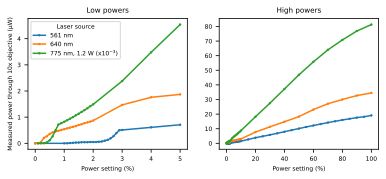
\includegraphics{laser_power}
	\caption{
		The power of each of the three lasers as measured through a 10x objective. Notice the non-linearity at low power settings. The 775 nm data was scaled down by three orders of magnitude.
	}
	\label{fig:laser power}
\end{figure}

\begin{figure}
	\centering
	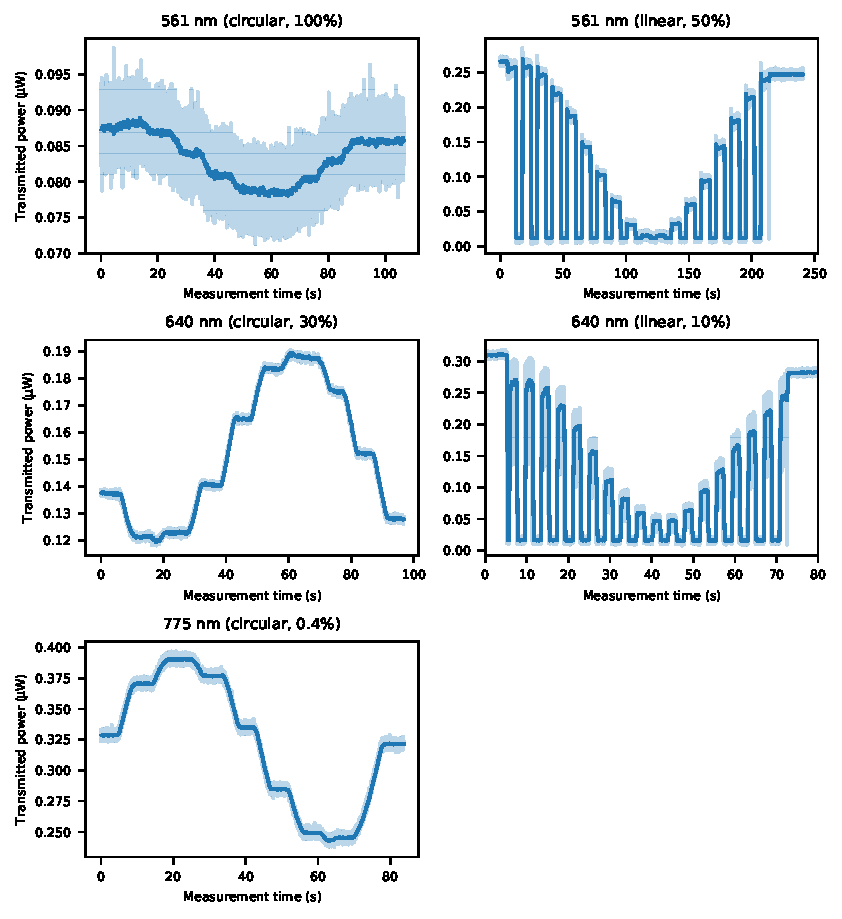
\includegraphics{laser_polarisation}
	\caption{
		Polarisation characterisation of the different lasers. To characterise circular polarisation, a polariser was placed in the sample and scanned from \ang{0} to \ang{180} in steps of \ang{20} (notice that I forgot to sample \ang{260} in the 775 nm data). Linear polarisation was characterised by fixing the polariser in place at \ang{0} and scanning the laser itself from \ang{0} to \ang{180} in steps of \ang{10}. Dark blue: average over 200 samples, light blue: raw data.
	}
	\label{fig:laser polarisation}
\end{figure}

\begin{figure}
	\centering
	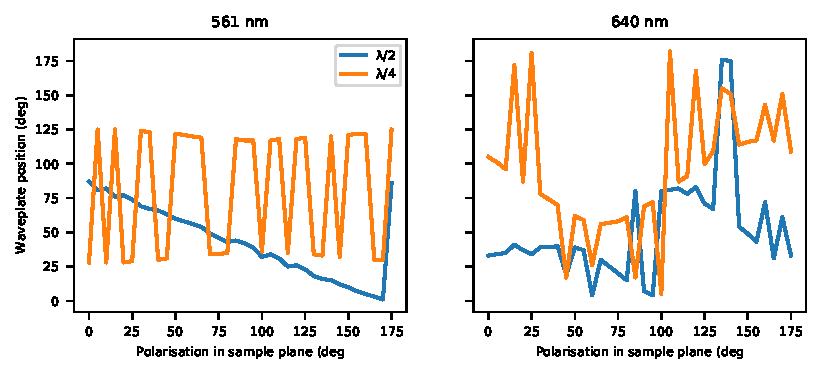
\includegraphics{excitation_waveplate_calibrations.pdf}
	\caption{
		Calibrations of the excitation waveplates, as supplied by the microscope manufacturer.
	}
	\label{fig:excitation waveplate calibration}
\end{figure}

\begin{figure}
	\centering
	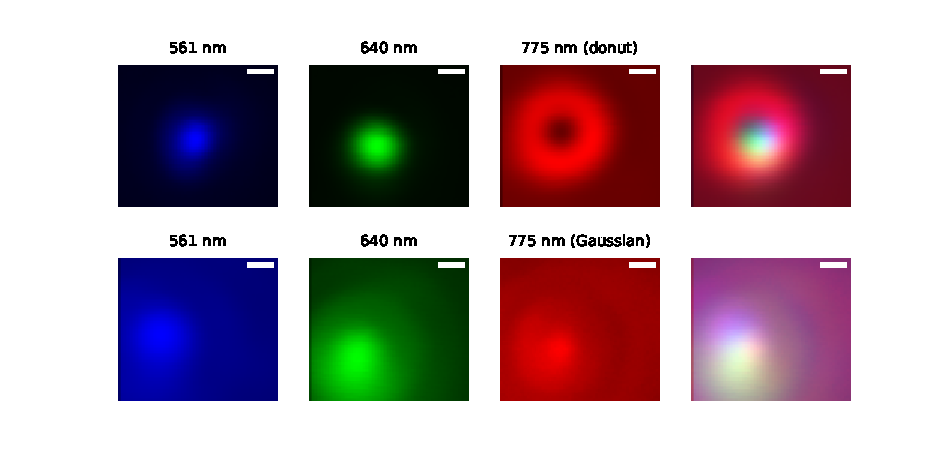
\includegraphics{laser_psfs.pdf}
	\caption{
		Point spread functions of the different lasers (in donut and Gaussian modes) at different SLM configurations, by measuring the reflection from 100 nm wide gold beads. Scale bars 200 nm.
	}
	\label{fig:normal psfs}
\end{figure}

\begin{figure}
	\centering
	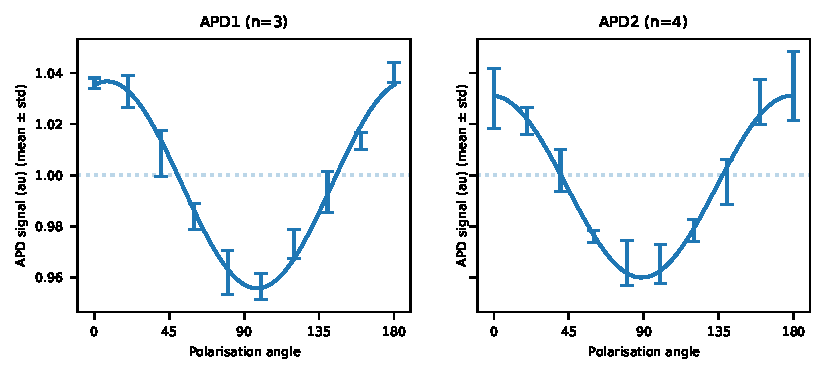
\includegraphics{apd_pol_sensitivity.pdf}
	\caption{Dependence of the signal from APD1 on the angle of polarisation of incoming light.}
	\label{fig:apd pol sensitivity}
\end{figure}

\begin{figure}
	\centering
	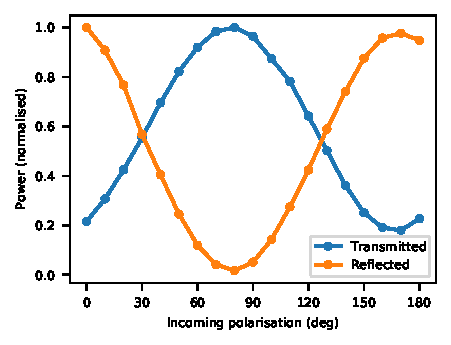
\includegraphics{pol_cube.pdf}
	\caption{Performance of the polarising beam splitter.}
	\label{fig:pol cube}
\end{figure}

\begin{figure}
	\centering
	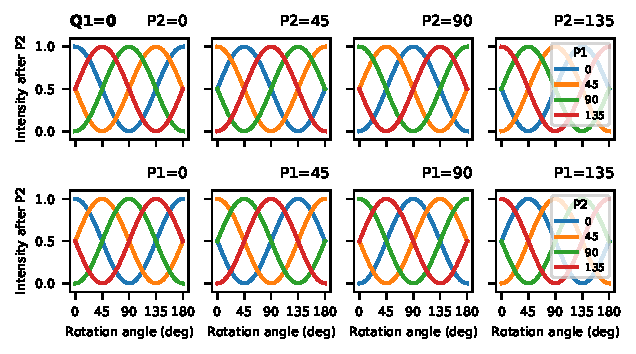
\includegraphics[scale=.95]{p1_effects_qwp_aligned.pdf}
	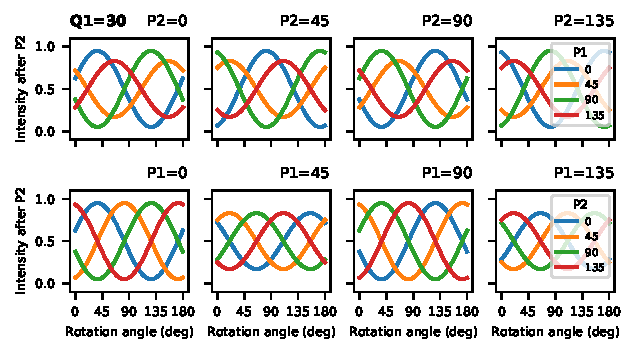
\includegraphics[scale=.95]{p1_effects_qwp_30.pdf}
	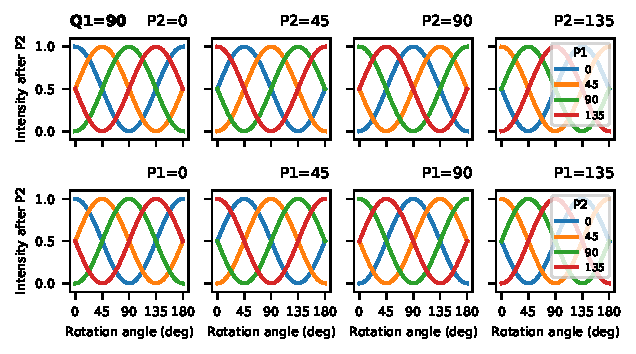
\includegraphics[scale=.95]{p1_effects_qwp_90.pdf}
	\caption{
		Simulation of the effect of QWP alignment on the action of the detection pathway. Shown are three simulations in which the first QWP is rotated by 0, 30, and 90 degrees, respectively. The second QWP is always rotated by 0, and the HWP is rotated to half the rotation angle (x-axis). When the QWPs have an offset of 90 degrees (bottom), the upper and lower panels (with either P1 or P2 constant) are identical, but when they are aligned (top), there is a phase difference. When they are not aligned at all (middle), intensity variations are prominent. This simulation is based on \autoref{eq:detection waveplates}.
	}
	\label{fig:detection waveplate simulations}
\end{figure}

\begin{figure}
	\centering
	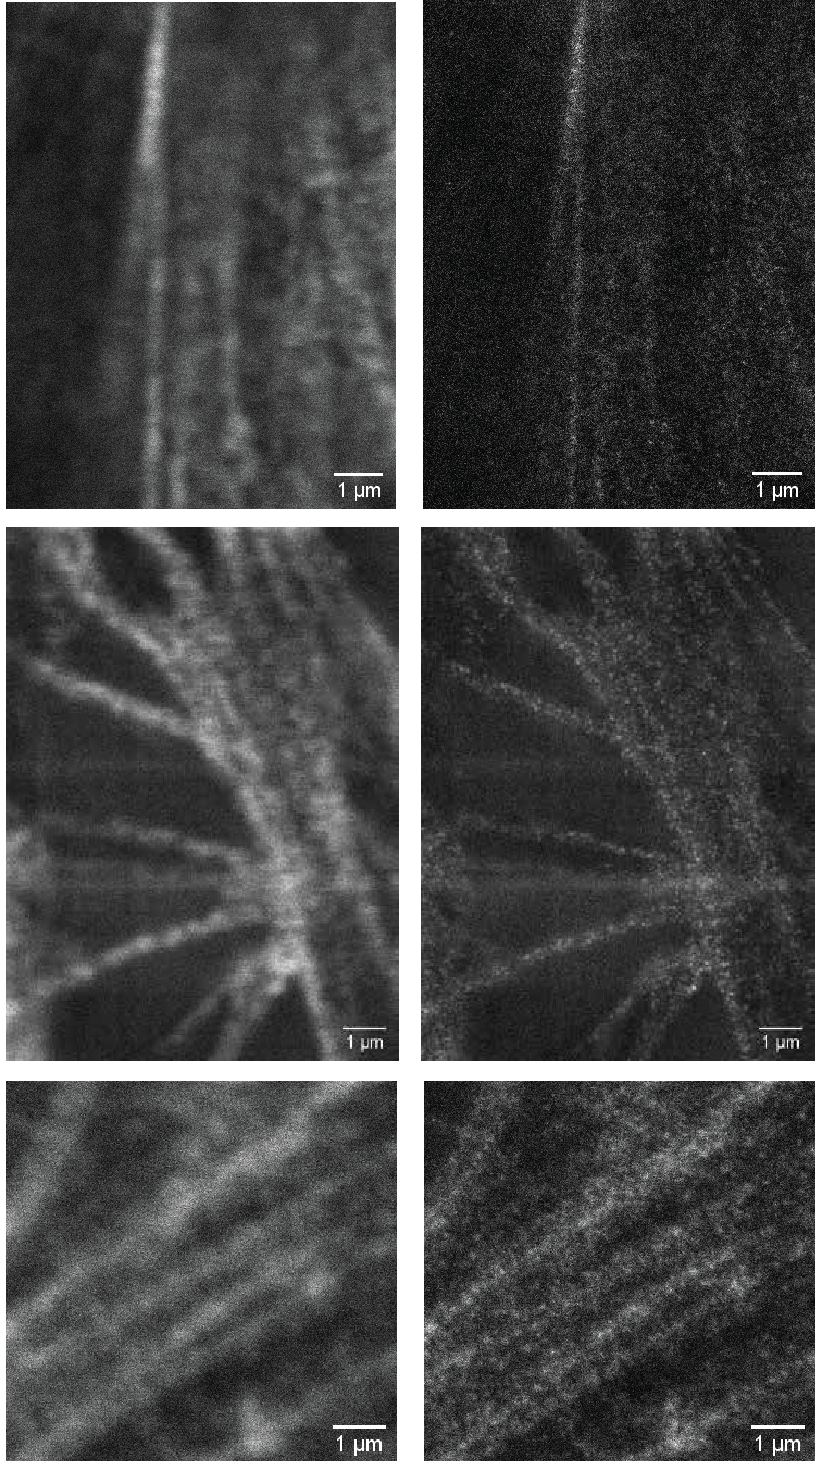
\includegraphics[width=.8\linewidth]{ssted_1.ai}
	\caption{
		Confocal (left) and STED (right) acquisitions of various fields of view.
	}
	\label{fig:ssted supplementary}
\end{figure}


\begin{figure}
	\centering
	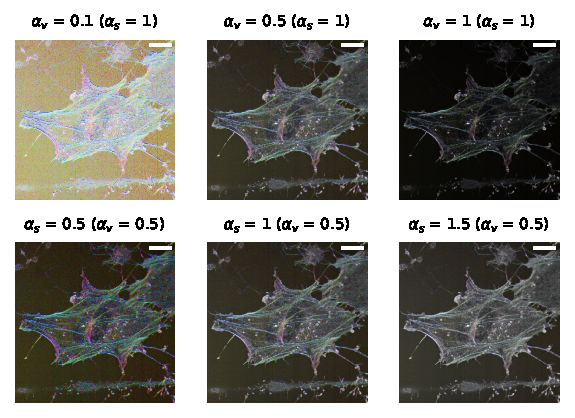
\includegraphics{conventional_pol.pdf}
	\caption{
		The effect of the exponents $ \alpha_s $ (tuning saturation) and $ \alpha_v $ (scaling brightness) on an image.
	}
	\label{fig:power law exponents}
\end{figure}

\begin{figure}
	\centering
	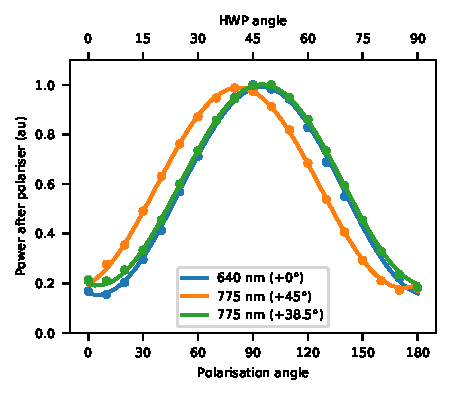
\includegraphics{psted_hwp_offset.pdf}
	\caption{
		The rotating HWP I put in the beamline controls the depletion beam polarisation. With an offset of 38.5°, the depletion beam is parallel to the 640 laser (set to vertical linear polarisation).
	}
	\label{fig:psted hwp offset}
\end{figure}

\begin{figure}
	\centering
	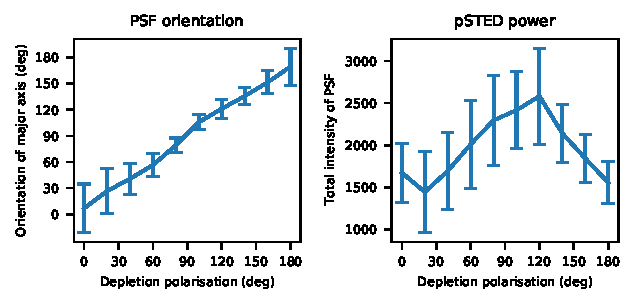
\includegraphics{psted_psfs_orientation_and_power.pdf}
	\caption{
		\textbf{Left:} The pSTED PSF is elliptical, and its orientation matches the light polarisation. \textbf{Right:} pSTED intensity depends on polarisation. Error bars show standard deviation, n=10.
	}
	\label{fig:psted psf orientation and power}
\end{figure}

\begin{figure}
	\centering
	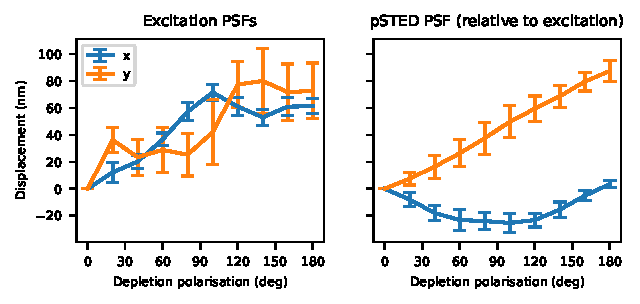
\includegraphics{psted_psfs_displacement.pdf}
	\caption{
		The displacement of the laser PSFs as a function of depletion polarisation. \textbf{Left:} The displacement of the 561~nm and 640~nm PSFs (representing drift in the image). \textbf{Right:} Displacement of the pSTED PSF relative to the excitation PSFs.
	}
	\label{fig:psted displacement}
\end{figure}